\documentclass[tikz, border=1mm]{standalone}
\usetikzlibrary{bayesnet}
\usetikzlibrary{positioning}

\begin{document}
    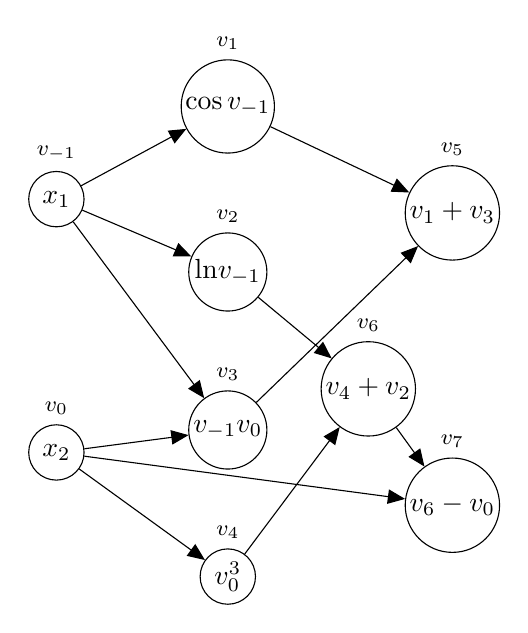
\begin{tikzpicture}
        % Define nodes
        % measurements
        \node[latent, label=above:{$v_{-1}$}](v_m1){$x_1$}; %
        \node[latent, below=2.5cm of v_m1,label=above:{$v_{0}$}](v_0){$x_2$}; %
        \node[latent, above right =0.5cm and 1.5cm of v_m1, label=above:{$v_{1}$}](v_1){$\cos v_{-1}$}; %
        \node[latent, below=of v_1,label=above:{$v_{2}$}](v_2){$\mathrm{ln}v_{-1}$}; %
        \node[latent, below=of v_2,label=above:{$v_{3}$}](v_3){$v_{-1}v_0$}; %
        \node[latent, below=of v_3,label=above:{$v_{4}$}](v_4){$v_{0}^3$}; %
        \node[latent, below right =0.5 cm and 2cm of v_1,label=above:{$v_{5}$}](v_5){$v_1+v_3$};
        \node[latent, below right =0.7 cm and 1cm of v_2,label=above:{$v_{6}$}](v_6){$v_4+v_2$};
        \node[latent, below=2.5 cm of v_5,label=above:{$v_{7}$}](v_7){$v_{6}-v_0$}; %

        \edge{v_m1}{v_1,v_2,v_3};
        \edge{v_0}{v_3,v_4};
        \edge{v_2,v_4}{v_6};
        \edge{v_1,v_3}{v_5};
        \edge{v_6,v_0}{v_7};

        % \node[latent, right=of v_0,label=above:{$v_1$}](v_1){$v_0^2$}; %
        % \node[latent,right=of v_1,label=above:{$v_2$}](v_2){$5v_1$}; %
        % \node[latent,right=of v_2,label=above:{$v_3$}](v_3){$\cos v_2$}; %
        % \edge {v_0} {v_1} ;
        % \edge {v_1} {v_2} ;
        % \edge {v_2} {v_3} ;       
    \end{tikzpicture}
\end{document}